\bluepage{Konfigurace Vertex Pulleru/Vertex Array Object}

\begin{frame}
\frametitle{Vertex Array Object}
  \begin{itemize}
  \item Vertex Array Object (VAO) obsahuje konfiguraci Vertex Puller jednoty.
  \item Vertex Puller čte data z bufferů a plní je do vstupních proměnných v prvním shaderu (vertex shader)
  \item VAO obsahuje nastavení propojení Shader Programu a Bufferů
  \item V novějších verzích OpenGL je povinný
  \item Obsahuje sadu nastavení pro každý Vertex Attribut a nastavení pro indexový buffer
  \item Jeden Vertex Attribut je napojen na jednu vstupní proměnnou ve Vertex Shaderu
  \item Mezi nastavení Vertex Attributu patří: číslo bufferu, velikost a typ datové položky, prokládání (stride), offset
  \end{itemize}
\end{frame}

\begin{frame}
\frametitle{Příklad - ilustrace 0. invokace vertex shaderu}
  \begin{figure}[h]
  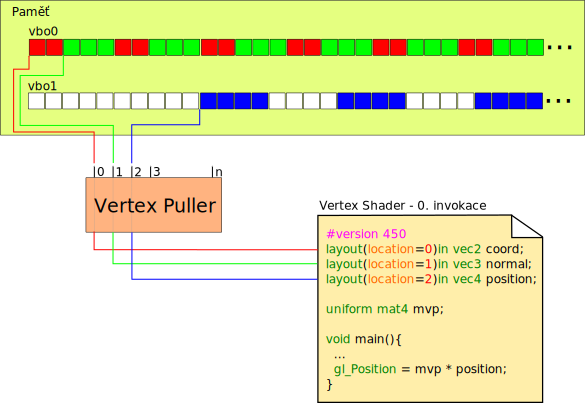
\includegraphics[width=10cm,keepaspectratio]{pics/vao/puller0.pdf}
  \end{figure}
\end{frame}

\begin{frame}
\frametitle{Příklad - ilustrace 1. invokace vertex shaderu}
  \begin{figure}[h]
  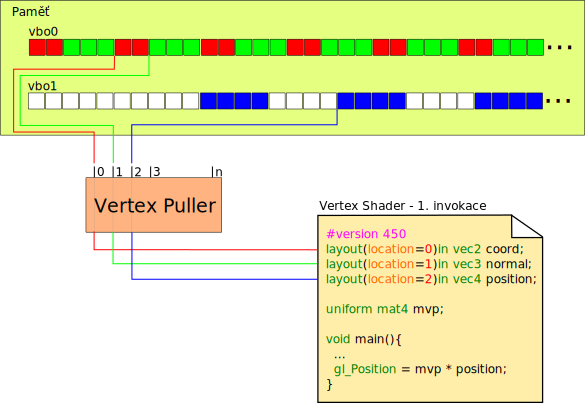
\includegraphics[width=10cm,keepaspectratio]{pics/vao/puller1.pdf}
  \end{figure}
\end{frame}

\begin{frame}[fragile]
\frametitle{VAO - příklad}
{\scriptsize
\begin{minted}[bgcolor=bg]{packages/c_cpp.py:CppLexer -x}
GLuint vao;
glCreateVertexArrays(1,&vao);//vygenerovani jmena VAO
//nyni nastavime buffery a atributy

glVertexArrayAttribBinding(vao,0,0);
glEnableVertexArrayAttrib(vao,0);
glVertexArrayAttribFormat(vao,
  0,//cislo vertex attributu
  2,//pocet polozek pro cteni (vec2)
  GL_FLOAT,//typ polozek
  GL_FALSE,//normalizace
  0);//relativni offset
glVertexArrayVertexBuffer(vao,0,
  vbo,
  sizeof(float)*5,//stride
  (GLvoid*)(sizeof(float)*0));//offset

glVertexArrayAttribBinding(vao,1,1);
glEnableVertexArrayAttrib(vao,1);
glVertexArrayAttribFormat(vao,1,3,GL_FLOAT,GL_FALSE,0);
glVertexArrayVertexBuffer(vao,1,vbo,sizeof(float)*5,
  (GLvoid*)(sizeof(float)*2));

glVertexArrayAttribBinding(vao,2,2);
glEnableVertexArrayAttrib(2);
glVertexArrayAttribFormat(2,4,GL_FLOAT,GL_FALSE,0);
glVertexArrayVertexBuffer(vao,2,vbo,sizeof(float)*8,
  (GLvoid*)(sizeof(float)*10));
\end{minted}
}
\end{frame}

\begin{frame}[fragile]
\frametitle{VAO}
  \begin{figure}[h]
  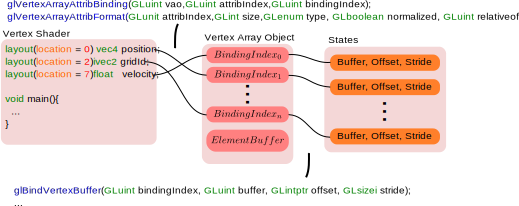
\includegraphics[width=11cm,keepaspectratio]{pics/vao/vao.pdf}
  \end{figure}
\end{frame}

